%%%%%%%%%%%%%%%%%%%%%%%%%%%%%%%%%%%%
% This is the template for submission to HPCA 2019
% The cls file is a modified from  'sig-alternate.cls'
%%%%%%%%%%%%%%%%%%%%%%%%%%%%%%%%%%%%

\documentclass{sig-alternate}
\setlength{\paperheight}{11in}
\setlength{\paperwidth}{8.5in}

\newcommand{\ignore}[1]{}
\usepackage[pass]{geometry}
\usepackage{fancyhdr}
%\usepackage[normalem]{ulem}
%\usepackage[hyphens]{url}
%\usepackage{hyperref}
\usepackage{color}
\usepackage{soul}

%%%%%%%%%%%---SETME-----%%%%%%%%%%%%%
\newcommand{\hpcasubmissionnumber}{6}
%%%%%%%%%%%%%%%%%%%%%%%%%%%%%%%%%%%%
%\sethlcolor{white}

%%%%%%%%%%% NADER: %%%%%%%%%%%%
\usepackage{xspace}
\usepackage{xcolor}
\usepackage{textcomp}
\usepackage{siunitx}
\usepackage[hyphens]{url}

\usepackage{listings}
\usepackage[breaklinks,colorlinks]{hyperref}
\hypersetup{citecolor=blue,linkcolor=blue}
%\def\sectionautorefname{Section}
%\def\subsectionautorefname{SubSection}

\renewcommand{\sectionautorefname}{\S}
\renewcommand{\subsectionautorefname}{\S}
%\usepackage[subpreambles=true]{standalone} 
\usepackage{pgfplots}
\usepackage{filecontents}
\usepackage{tikz}
\usetikzlibrary{arrows,calc}
\usetikzlibrary{patterns}
\usepackage{relsize}
\usepackage{tikz-cd}
%%
\usepackage{color}
\usepackage{enumitem}
\setlist{leftmargin=1em}

\definecolor{codegreen}{rgb}{0,0.6,0}
\definecolor{codegray}{rgb}{0.5,0.5,0.5}
\definecolor{codepurple}{rgb}{0.58,0,0.82}
\definecolor{backcolour}{rgb}{0.95,0.95,0.92}
\definecolor{backwhite}{rgb}{0.95,0.95,0.95}

\definecolor{mycolor}{rgb}{1,0,0}


\lstdefinestyle{mystyle}{
  backgroundcolor=\color{backwhite},   
  commentstyle=\color{codegreen},
  keywordstyle=\color{magenta},
  numberstyle=\tiny\color{backcolour},
  stringstyle=\color{codepurple},
  basicstyle=\footnotesize,
  breakatwhitespace=false,         
  breaklines=true,                 
  captionpos=b,                    
  keepspaces=true,                 
  numbers=left,                    
  numbersep=5pt,                  
  showspaces=false,                
  showstringspaces=false,
  showtabs=false,                  
  tabsize=2
}

\lstset{style=mystyle}

\renewcommand{\lstlistingname}{Example}

%%
\newcommand{\iot}{CPS\xspace} % IoT changed to CPS




% When sethlcolor is white, your highlights will not show up.  Use
% \sethlcolor{white} to submit your paper pdf.  When compiling your second
% pdf with highlighted changes, simply remove \sethlcolor{white} and add your
% optional 100-word appendix.
% Use \hl{ ... } to highlight any text.
%%%%%%%%%%%%%%%%%%%%%%%%%%%%%%%%%%%%

\fancypagestyle{firstpage}{
  \fancyhf{}
\setlength{\headheight}{50pt}
\renewcommand{\headrulewidth}{0pt}
  \fancyhead[C]{\normalsize{HPCA 2019 Industrial Track Submission
      \textbf{\#\hpcasubmissionnumber} -- Confidential Draft -- Do NOT Distribute!!}}
  \pagenumbering{arabic}
}

%%%%%%%%%%%---SETME-----%%%%%%%%%%%%%
\title{Understanding the Impact of ISAs on Performance and Power of Modern Embedded Systems}
%%%%%%%%%%%%%%%%%%%%%%%%%%%%%%%%%%%%

\begin{document}
\maketitle
\thispagestyle{firstpage}
\pagestyle{plain}



%%%%%% -- PAPER CONTENT STARTS-- %%%%%%%%

\begin{abstract}

  %% abstract


Instruction Set Architecture (ISA) is fundamental to how a wide variety of modern computer systems -- ranging from simple handheld mobile devices to large scale data centers -- are conceived, designed and implemented. One of the primary goals of ISA designers is to capture the most basic functions and tasks that can be used as basic building blocks to compose and express complex applications and softwares. The general expectation is that a computing system should perform these functions in most efficient manner in terms of performance, power, energy and area. 

While an ISA is central to computer design, there have been only a handful of successful ISAs till date. This limits designers' options and forces them to rely on a small subset even though it might not be efficient in capturing appropriate necessary functions needed for higher level applications. Unlike compilers, OSs, drivers, and other software components, ISAs have been a proprietary component by-and-large.

``Democratization of ISA'' was the main theme behind the advent of RISC-V with overarching goal to relieve the designer community and small- to mid-scale OEMs from the clutches of proprietary ISA suppliers. While this is a novel thought in spirit, in reality, much depends upon the efficacies of democratized ISA effort and the eventual ecosystem. In this work, we set out to discern and quantify the viability of an open source ISA such as RISC-V. We conduct numerous program and microarchitectural analysis on major RISC ISAs (ARM, MIPS and RISC-V) and present our findings. Overall, while RISC-V being a promising start so far, there is still a lot needs to be done to fully democratize ISA component.  

\vspace{0.5em}
\noindent
\textbf{Keywords:} RISC-V, ARM, MIPS, Performance, Power, Area, Energy, Program analysis, Microarchitecture.







\end{abstract}

\section{Introduction}

Numerous isas have been designed but couldn’t survive because they either didn’t offer anything unique or they were poorly designed.

RISCV is an emerging Instruction Set Architecture (ISA) and has become an important option for both academia and industry when considering new microprocessor designs. Features like modularity, extensibility, simplicity, and being open and free to use, make RISCV an attractive option for next generation of processors especially in embedded systems domain where new, customized, low-power, and efficient cores are needed.  In this paper we present a comparative study on impacts of three well-known Instruction Set Architectures (ISAs) (MIPS, ARM, and RISCV) on Performance, Power, and Area (PPA) of state-of-the-art embedded processors through a systematic measurement campaign using several different toolchains and frameworks and several standard benchmark suites.  We particularly study the impact of these ISAs on important metrics such as static and dynamic Instruction Count (\textit{icount}), Cycle Count, Microarchitectural Statistics (e.g. MPKI, Branch Prediction Accuracy, etc.), Dynamic Power, and Core's Area and report our key findings on impacts of using different ISAs on each of these metrics. We find that some of these metrics are ISA-dependent and others are dependent on other factors such as compiler, runtime libraries, and specific microarchitectural features. Our main conclusion is that while comparing to MIPS and ARM, RISCV has some shortcomings and design/toolchain issues that should be addressed and fixed, due to its intrinsic features such as modularity it provides a great opportunity for designing customized PPA-efficient cores.   

Instruction Set Architectures (ISAs) has a key role in designing cores for different domains, where x86 ISA has become dominant in desktop and server domains, and ARM has become the dominant ISA in mobile, tablet, and embedded system domain. The question of impact of ISA design on different Performance, Power, Area (PPA) metrics has traditionally been an important concern for designers and semiconductor industry especially in the 1980s and 1990s when
chip area and processor design complexity were the primary
constraints [24, 12, 17, 7]. In the past decade, we radical changes in computing landscape and rise of mobiles and tables and increasing popularity of ARM ISA this question again becomes an important issue. 

Today, with proliferation of embedded and cyber-physical systems (e.g. IoTs) and increasing popularity of domain-specific languages and emerging applications like machine-learning and more importantly, introduction of a new, open-source, modular ISA (RISCV), this question once again becomes an interesting topic for research. 

To answer this question, in this paper we present a comparative study on impacts of using three different ISAs (MIPS, ARM, and RISCV) on important metrics such as static and dynamic instruction count (icount), total execution time (cycle count), dynamic power, and area. We show which of these metrics are ISA-dependent and what are the other important factors on PPA. Using these experiments we pinpoint the shortcomings, issues, and advantages of using RISCV ISA over ARM and MIPS ISAs. 




\section{Background}

\label{sec:bak}
RISC-V is an emerging open-source software and hardware ecosystem that has gained in popularity in both industry and academia [2, 11]. At the heart of the ecosystem, the RISC-V ISA is designed to be open, simple, extensible, and free to use. The RISC-V software tool chain includes open-source compilers (e.g., GNU/GCC and LLVM), a full Linux port, a GNU/GDB debugger, verification tools, and simulators. On the hardware side, several RISC-V prototypes (e.g., Celerity [4]) have been published. The rapid growth of the RISC-V ecosystem enables computer architects to quickly leverage RISC-V in their research.




\section{Methodology}

\label{sec:method}

\newcommand{\icount}{\textsc{icount}\xspace}

To study the effects of ISAs on Power, Performance, and Area, we used several different metrics using 4 different tools and more than 12 standard benchmark applications. Followings describe the frameworks, metrics, and benchmarks used in this paper. The reader can skip this section if he/she is uninterested in these details. 

\subsection{ISAs and Compiler}
Table~\ref{t:isa} shows the ISAs used in study. For each of these ISAs, we use \textit{gnu-gcc} cross-compiler. We intentionally chose gcc so
that we can use the same front-end to generate all binaries. All
target independent optimizations are enabled (O3); machine specific
tuning is disabled so there is a single set of binaries for each ISA. For MIPS, \textit{-march} is used to generate MIPS release 6, 32bit and 64bit versions. For ARM, two separate compilers ARMv7 and AARCHv8 are used to generate 32bit and 64bit ARM binaries. Finally, for RISCV we use the gnu-toolchain provided by RISCV developers publicly available in github. We believe using similar flags and front-end could help us to mitigate the effect of compilers on performance and power metrics, however, we will later show that RISCV compiler does have important inefficiencies and issues that could hurt the performance of the system. 

\begin{table}[h]
\centering
\caption{ISAs used in this study.}
\begin{tabular}{|c|c|}
\hline
%\multicolumn{3}{ |c| }{Team sheet} \\
\small \textbf{ISAs} & \small \textbf{Specification} \\
\hline \hline
\small ARM & \small  32v7, 64v8 (AARCH) \\
\hline
\small MIPS & \small 32r6, 64r6 \\
\hline
\small RISCV &\small  rv32g (IMAFD), rv64g \\
\hline
\end{tabular}
\label{t:isa}
\end{table}

\subsection{Framework} 
\subsubsection{QEMU}
To find the dynamic and static instruction count (\icount), we use a well-known open-source emulator called QuickEMUlator (QEMU). QEMU is a hosted virtual machine monitor: it emulates the machine's processor through dynamic binary translation and provides a set of different hardware and device models for the machine, enabling it to run a variety of guest operating systems. We chose QEMU primarily cause it can emulates MIPS, ARM, and RISCV ISAs in user-mode. 



\noindent \textbf{Static Instruction Count}: Static icount is a classic metric to show the code density of different ISAs which can directly affect the performance, power, and area (i.e. required icache size). While static icount can simply be measured by measuring the lines of assembly code in a binary, a more meaningful and useful way to measure this metric is to count number of unique PCs (each PC represents an instruction) seen during the execution of the an application (i.e. counting only those instructions that are actually executed at least once). We believe this approach provides a better insight on the actual instruction memory footprint and shows the difference between ISAs better. We found that these two number (our approach vs. measuring the size of the code) could be quite different for some applications since compilers might include source codes for all routines in an included library, while some of these routines may not be used at all.  

To find static icount, we modified QEMU's source code to add a new data structure to track and count unique PCs during the execution. These changes are made in a routine called \textsc{exec\_cpu()} which is used in all ISAs. To check the correctness of our model, for each ISA, we used several synthetic benchmarks and checked the QEMU's output to the actual static icount computed manually. 

\noindent \textbf{Dynamic Instruction Count}: Similar to static icount, dynamic icount is also an important metric to show the runtime behavior of ISAs. Dynamic icount can directly affect total runtime especially in simple in-order cores where Instruction Per Cycle (IPC) for these cores are mostly close to 1 thus the total runtime is determined by dynamic icount metric. 

Dynamic icount is also computed in QEMU by modifying the source code to be able to count this metric during execution. The results are validated using a synthetic benchmark where number of iterations of a simple loop changed in different runs. We checked whether QEMU correctly reports dynamic icount as the number of iterations changed for each run. 

\noindent \textbf{Per-PC Iteration Count}: Another interesting metric which used in this paper is per-PC iteration count where for each PC we report how many times this instruction has been executed. This could be very useful to find the hot regions in the code, and find the reason(s) behind why some applications have significantly higher/lower dynamic icount. More details will be shown in the Section ??. QEMU is modified to count this metric too, during execution. 

\subsubsection{gem5}
gem5 is a well-known, open-source, cycle-accurate simulator which can simulate in-order and out-of-order cores, memory systems, and interconnect in details. Using gem5 enables us to find runtime statistics (e.g total number of cycles) and micro-architecture related statistics (e.g. cache miss rate). gem5 supports ARM and very recently RISCV. Unfortunately gem5 only supports an old version of MIPS and hence we removed the analysis for MIPS in gem5. To have a fair comparison, processor and memory system configurations (i.e. clock rate, issue width, cache levels and size, delays, etc.) are matched for both ARM and RISCV processors. We use a simple single-issue, 4-stage pipeline with no prefetcher and a single-level cache as an in-order core for RISCV and ARM, and use a more sophisticated 4-issue, out-of-order, with a direct/indirect prefetcher and two level caches as an out-of-order core in our experiments. Detailed for these two cores are shown in Table~\ref{t:config}.

\begin{table}[h]
\caption{Simulation configuration for gem5.}
\begin{tabular}{|c|c|c|}
\hline
%\multicolumn{3}{ |c| }{Team sheet} \\
\small \textbf{Parameters} &\small \textbf{In-order core} &\small \textbf{Out-of-Order core} \\
\hline \hline
\small Issue Width & \small 1 & \small 4 \\
\hline
\small Private Caches & \small I\$/D\$ 32KB & \small I\$/D\$ 32KB\\
\hline
\small Shared Caches & \small N/A & \small L2 256KB \\
\hline
\small Branch Predictor & \small N/A & \small Tournament BP and BTB \\
\hline
\small Prefetcher & \small N/A & \small stride/next-line prefetcher \\
\hline
\end{tabular}
\label{t:config}
\end{table}

\noindent \textbf{Cycle Count and IPC}: we use the number reported by gem5 for these metrics. Same input is used for both RISCV and ARM and the numbers reported are from beginning to end of each application. We use IPC to show the effect of using different ISAs on processor's computation speed. Our key findings about these two numbers will be shown in Section ??. 

\noindent \textbf{Microarchitecture Statistics}: to gain some insights about the runtime behavior of each core and ISA's impacts on them, we check several microarchitecture-related metrics such as: cache miss rate (MPKI), branch predictor accuracy, instruction mix, fetch and commit rates, total stall/idle/squashed cycles, memory bandwidth utilization, direct/indirect branches and function calls, and dependent memory load/stores across different applications. 

\subsubsection{McPAT}
McPAT is an integrated power and area modeling simulator. It uses ITRS roadmap models at circuit level to model both static and dynamic power of the system. McPAT uses an XML-based interface to read microarchitecture-related statistics generated by a cycle-accurate simulator (e.g. gem5) as inputs and uses a detailed model for cores, memory system, NoC, etc. to estimate the area and power of the system. We use a set of python and shell scripts to parse the statistics from gem5 and fill in the XML template in McPAT.  

\noindent \textbf{Dynamic Power and Total Energy}: using McPAT, we measure the dynamic power consumption of core (both in-order and out-of-order) and memory system. Using the data from gem5, we also calculate the overall energy for these ISAs.

\subsection{Applications}
We use a representative set of applications from a standard open-source embedded system's benchmark suite called MiBench. The MiBench suite is commonly used to evaluate the performance of processors intended for the embedded/IoT market, and it was designed to be representative of the computation that is needed in that market (e.g. automotive, industrial systems, etc.). These applications are mostly compute intensive and designed such that have minimum interactions with outside the processors. Many of the applications are also overlapped with EEMBC benchmark suite. 

Our applications we picked ranges from basic math abilities (\textit{basicmath}), bit manipulation (\textit{bitcount}), simple data organization (\textit{qsort}), a shape recognition program (\textit{susan}), shortest path calculations (\textit{dijkstra}), to data encryption, decryption and hashing (\textit{blowfish, rijandael, sha}), and communications applications (\textit{fft, crc32, adpcm}). In addition to these 11 applications picked from MiBench, we use two well-known open-source application which often used in industry to report the performance of the processor \textit{Coremark} and \textit{Dhrystone}. For each of these applications the ``large'' dataset is used. For Coremark and Dhrystone, iterations are chosen such that the total number of executed instructions be more than 200 million instructions (we chose 1000 iterations for Coremark and 1 million iterations for Dhrystone). For each application, same inputs are used for all runs across different ISAs/processors. 

   
 


\section{Experimental Results and Analysis}
In this section we report our results and findings of static and dynamic instruction count, performance, power, and energy. 

\subsection{Instruction Count}
Figure~\ref{fig:static} shows the static icount obtained from QEMU. As seen in the figure, on average 32bit and 64bit ARM are about 15\% more dense than that of in MIPS and RISCV. Mibench applications have on average 5k instruction that are executed at least once. Figure~\ref{fig:dynamic} shows the dynamic icount obtained from QEMU. Unlike static icount, dynamic icount can be quite different from one application to another for different ISAs. However, on average MIPS, ARM, and RISCV have almost same dynamic icount. 

\begin{figure*}[htb]
	\centering
	%\footnotesize
	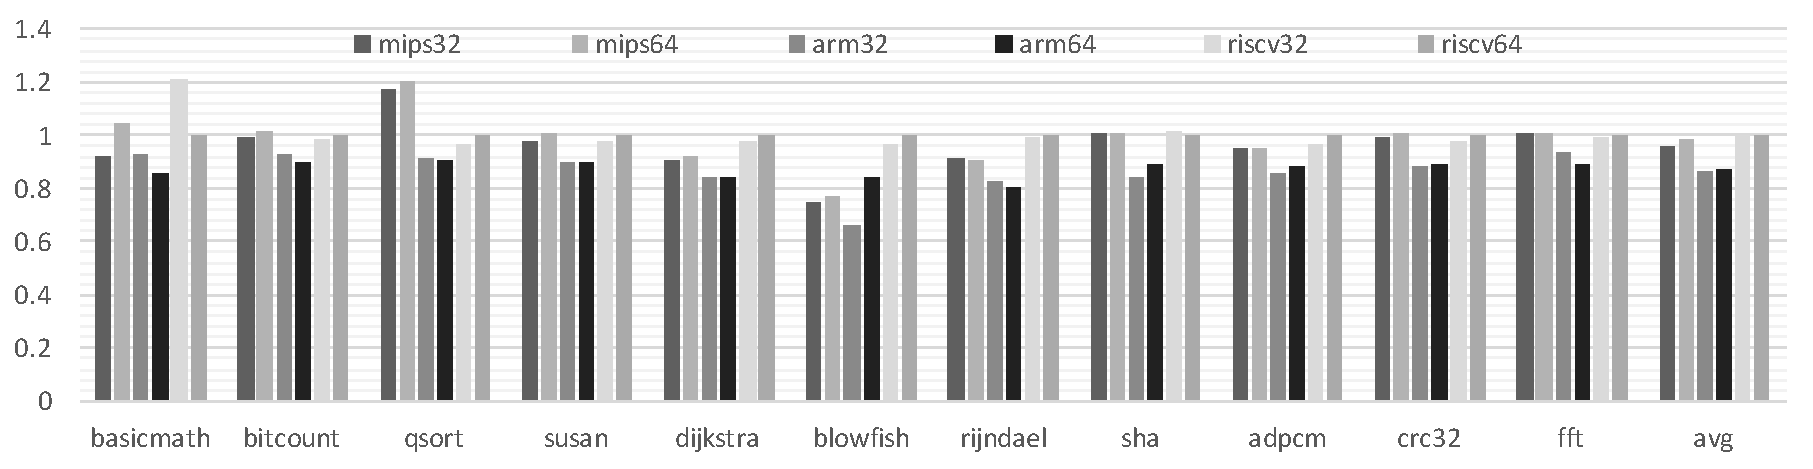
\includegraphics[width=1.8\columnwidth]{figures/static.pdf}
	\caption{Static Instruction Count for MiBench applications using QEMU. Results are normalized w.r.t. RISCV64. The average number of static instructions is about 5000 for these benchmarks.}
	\label{fig:static}
	%\vspace{-1em}
\end{figure*} 

\begin{figure*}[htb]
	\centering
	%\footnotesize
	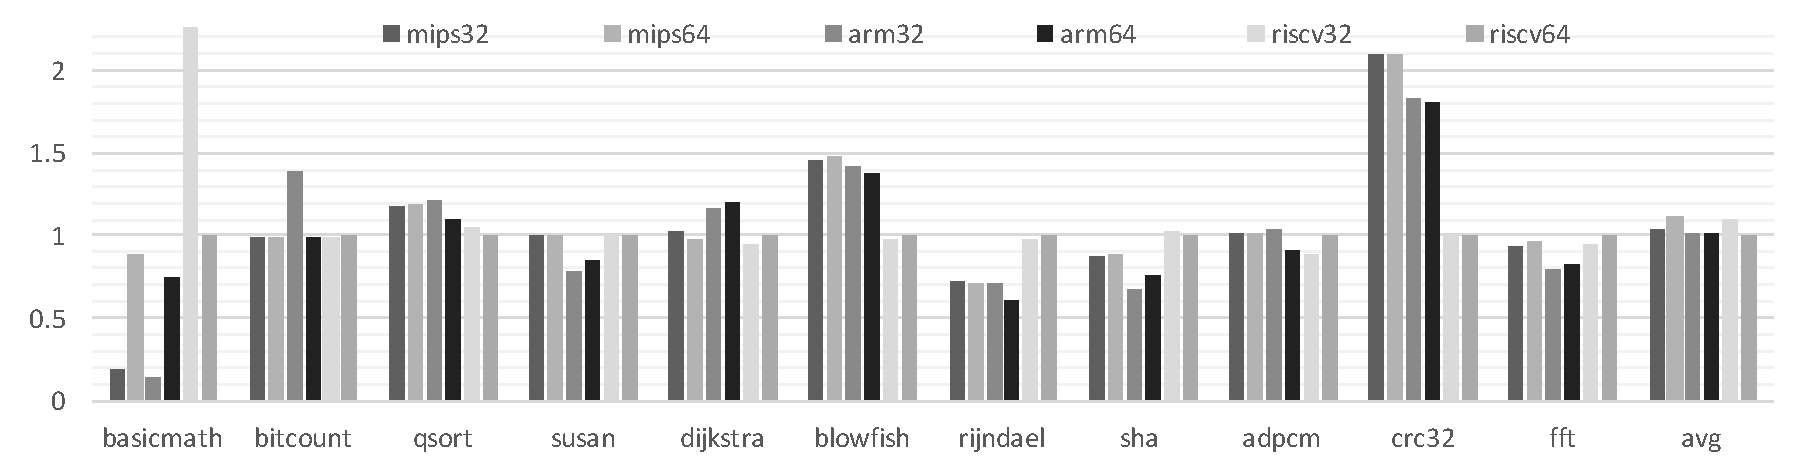
\includegraphics[width=1.8\columnwidth]{figures/dynamic.pdf}
	\caption{Dynamic Instruction Count for MiBench applications using QEMU. Results are normalized w.r.t. RISCV64. The average number of dynamic instructions for these benchmarks is about 450 million.}
	\label{fig:dynamic}
	%\vspace{-1em}
\end{figure*} 

\noindent \textbf{Key Findings}: 1- Mixed/Combined instructions (e.g. add+shift, mult+add, etc.) and three operand/three-way comparison in ARM could result in significant dynamic and static icount reduction. A possible and interesting extension to RISCV could be adding this sort of instructions to the base ISA (RV-G) for high-performance scenarios. An example is shown in Figure~\ref{fig:code}, where a same function is shown for ARM and RISCV ISAs. As seen in this example, ``ldr'' instruction in ARM with embedded ``lsl'' instruction inside it, has saved one instruction. Further ``cmn'' (compare and add), also saved two extra instructions in ARM. We found that there are many examples such as this where more complex instructions in ARM could save more space, however, we will later show that this complexity comes with more power consumption. 

\begin{figure}[t]
	\centering
	%\footnotesize
	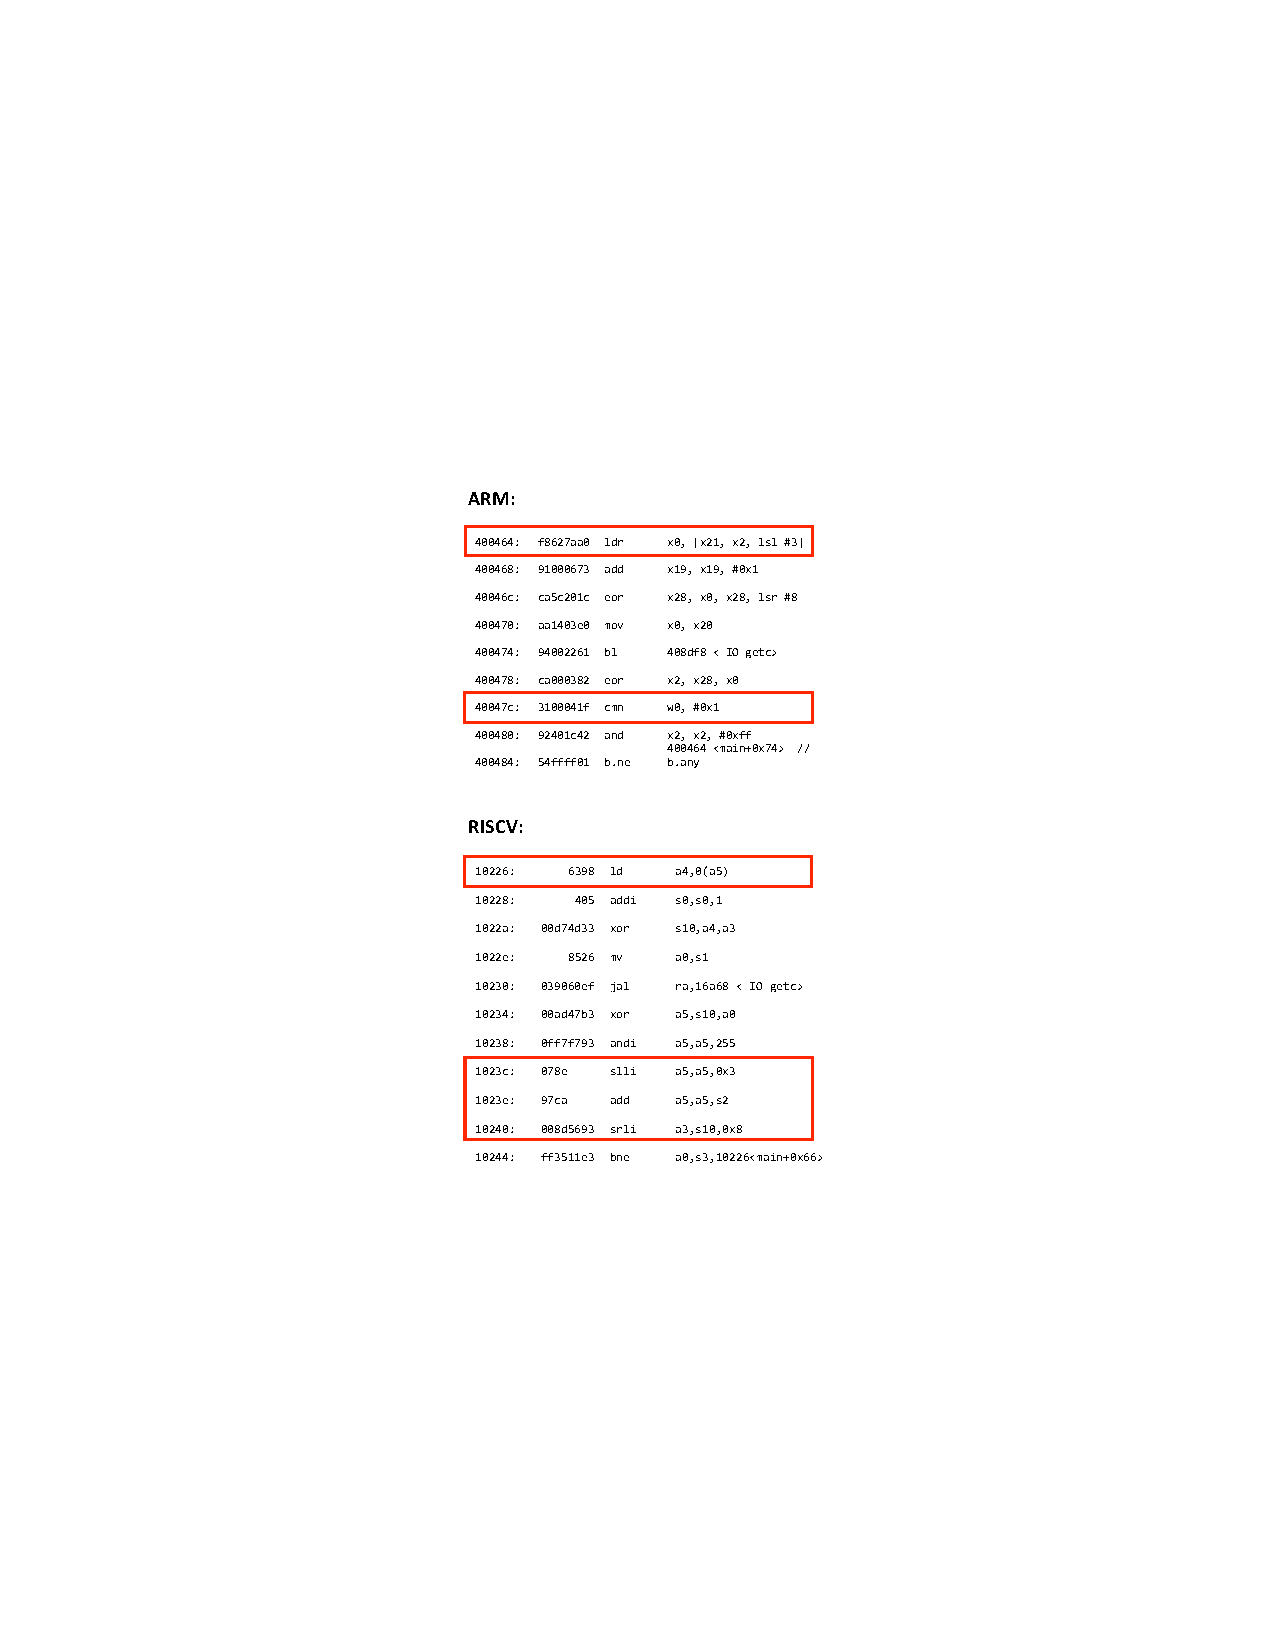
\includegraphics[width=0.9\columnwidth]{figures/code.pdf}
	\caption{A code snippet in assembly showing a same function from Mibench benchmark suite for ARM-64 and RISCV-64 ISAs. Differences shown in rectangles.}
	\label{fig:code}
	%\vspace{-1em}
\end{figure} 

\noindent \textbf{Outliers}: static icount for qsort on MIPS is significantly higher. The main reason for that is due to the way a hot loop in a function called \textsc{msort\_with\_temp} (part of glibc library for quicksort) is implemented in MIPS where a few extra instructions are used for MIPS. Interestingly, we find that this function is implemented slightly different among different toolchains. 


\section{Related Work}
%Early ISA studies are instructive but miss key changes in today’s
microprocessors and design constraints that have shifted the ISA’s effect. We review
previous comparisons in chronological order and observe that all prior comprehensive
ISA studies considering commercially implemented processors focused exclusively on
performance.
Bhandarkar and Clark compared theMIPS and VAX ISA by comparing theM/2000 to
the Digital VAX 8700 implementations [Bhandarkar and Clark 1991] and concluded:
“RISC as exemplified by MIPS provides a significant processor performance advantage.”
In another study in 1995, Bhandarkar compared the Pentium-Pro to the Alpha
21164 [Bhandarkar 1997], again focused exclusively on performance and concluded:
“the Pentium Pro processor achieves 80\% to 90\% of the performance of the Alpha
21164... It uses an aggressive out-of-order design to overcome the instruction set level
limitations of a CISC architecture. On floating-point intensive benchmarks, the Alpha
21164 does achieve over twice the performance of the Pentium Pro processor.” Consensus
had grown that RISC and CISC ISAs had fundamental differences that led to
performance gaps that required aggressive microarchitecture optimization for CISC
that only partially bridged the gap.
Isen et al. [2009] compared the performance of Power5+ to Intel Woodcrest considering
SPEC benchmarks and concluded that x86 matches the POWER ISA. The
consensus was that “with aggressive microarchitectural techniques for ILP, CISC and
RISC ISAs can be implemented to yield very similar performance.”
Many informal studies in recent years claim the x86’s “crufty” CISC ISA incursmany
power overheads and attribute the ARM processor’s power efficiency to the ISA.1 These
studies suggest that the microarchitecture optimizations from the past decades have
led to RISC and CISC cores with similar performance but that the power overheads of
CISC are intractable.
In light of the ISA studies from decades past, the significantly modified computing
landscape, and the seemingly vastly different power consumption of RISC implementations
(ARM: 1–2W, MIPS: 1–4W) to CISC implementations (x86: 5–36W), we feel there
is need to revisit this debate with a rigorous methodology. Specifically, considering the
multipronged importance of the metrics of power, energy, and performance, we need to
compare RISC to CISC on those three metrics. Macro-op cracking and decades of research
in high-performance microarchitecture techniques and compiler optimizations
seemingly help overcome x86’s performance and code-effectiveness bottlenecks, but these approaches are not free. The crux of our analysis is the following: After decades
of research to mitigate CISC performance overheads, do the new approaches introduce
fundamental energy inefficiencies?

\section{Conclusions}


% This document provides instructions for submitting papers to the 25th
% International Symposium on High Performance Computer Architecture (HPCA), 2019.  In an
% effort to respect the efforts of reviewers and in the interest of
% fairness to all prospective authors, we request that all submissions
% to HPCA 2019 follow the formatting and submission rules detailed
% below. Submissions that violate these instructions may not be reviewed,
% at the discretion of the program chairs, in order to maintain a review
% process that is fair to all potential authors.


% An example file (formatted using the HPCA'19 submission format) that
% contains the formatting guidelines can be downloaded from the 
% \href{http://hpca2019.seas.gwu.edu/}{HPCA webpage}.  The content of this
% document mirrors the submission instructions that appear on that
% page.  The link to the HotCRP submission site also appears on the HPCA
% webpage.

% All questions regarding paper formatting and submission should be directed
% to the program co-chairs using the email address hpca19@cs.utah.edu.

% \subsection{Format Highlights}
% Note that there are several notices for paper format:
% \begin{itemize}
% \item Paper must be submitted in printable PDF format.
% \item Text must be in a minimum 10pt ({\bf not} 9pt) font.
% \item Papers must be at most 11 pages, not including references. 
% \item No page limit for references.
% \item The references must include complete author lists (no {\em et al.}).
% \end{itemize}


% \subsection{Paper Evaluation Objectives}
% The committee will make every effort to judge each submitted paper on
% its own merits. There will be no target acceptance rate.
% We expect to accept a wide range of papers with appropriate expectations
% for evaluation --- while papers that build on significant past work
% with strong evaluations are valuable, papers that open new areas with
% less rigorous evaluation are equally welcome and especially encouraged.
% Given the wide range of topics covered by HPCA, every effort will be
% made to find expert reviewers.

% \subsection{Optional Second PDF for Resubmitted Papers}

% For submissions that were previously submitted to other conferences,
% we strongly encourage authors to take into account feedback received
% from previous reviews.  There is a reasonable probability that an
% HPCA-25 submission may be assigned to reviewers that have seen earlier
% versions of the same paper.  
% \hl{To ease the reviewing burden, and to help authors highlight the
% improvements to their paper, authors can optionally submit a second
% pdf that highlights the major changes to their work, relative to prior
% submissions.}
% We anticipate that this process will hold authors and reviewers more
% accountable, and perhaps help reduce any pre-conceived bias that a
% reviewer may have against the paper.
% \begin{itemize}
% \item The second pdf will not be made visible to reviewers by default.  If a reviewer believes they have reviewed an earlier version of the paper, they will email the PC Chairs and ask for the second pdf.
% \item The second pdf can not introduce new content.  It must be identical to the HPCA-25 submission, but can use color to highlight specific text/captions that are different from prior versions of the paper.  A 100-word appendix may be included to summarize and provide context for the major changes.
% \item In latex, text can be highlighted using \hl{ \textbackslash hl\{...\}, as has been done here.}  The submission template already includes the necessary latex packages color and soul.  To remove the highlight, simply set the highlight color to white (example in the latex template).
% \item Authors have the flexibility to decide what significant changes they want to highlight to a reviewer.  Obviously, authors will want to draw attention to all prior show-stopping concerns that have been addressed in the new submission.
% \item The second pdf upload deadline is also at 11:59pm EDT on Friday August 3rd.  For those planning on working on their paper until the last minute, a one hour grace period is being offered.
% \item In case of any questions about this new policy, please feel free to email the PC chairs at: \\ hpca19@cs.utah.edu.
% \end{itemize}


% \section{Paper Preparation Instructions}

% \subsection{Paper Formatting}

% Papers must be submitted in printable PDF format and should contain a
% {\bf maximum of 11 pages} of single-spaced two-column text, {\bf not
%   including references}.  You may include any number of pages for
% references, but see below for more instructions.  If you are using
% \LaTeX~\cite{lamport94} to typeset your paper, then we suggest that
% you use the template here:
% \href{http://hpca2019.seas.gwu.edu//hpca25-latex-template.tar.gz}{\LaTeX~Template}. This
% document was prepared with that template.  If you use a different
% software package to typeset your paper, then please adhere to the
% guidelines given in Table~\ref{table:formatting}.

% \begin{scriptsize}
% \begin{table}[h!]
%   \centering
%   \begin{tabular}{|l|l|}
%     \hline
%     \textbf{Field} & \textbf{Value}\\
%     \hline
%     \hline
%     File format & PDF \\
%     \hline
%     Page limit & 11 pages, {\bf not including}\\
%                & {\bf references}\\
%     \hline
%     Paper size & US Letter 8.5in $\times$ 11in\\
%     \hline
%     Top margin & 1in\\
%     \hline
%     Bottom margin & 1in\\
%     \hline
%     Left margin & 0.75in\\
%     \hline
%     Right margin & 0.75in\\
%     \hline
%     Body & 2-column, single-spaced\\
%     \hline
%     Space between columns & 0.25in\\
%     \hline
%     Body font & 10pt\\
%     \hline
%     Abstract font & 10pt, italicized\\
%     \hline
%     Section heading font & 12pt, bold\\
%     \hline
%     Subsection heading font & 10pt, bold\\
%     \hline
%     Caption font & 9pt (minimum), bold\\
%     \hline
%     References & 8pt, no page limit, list \\
%                & all authors' names\\
%     \hline
%   \end{tabular}
%   \caption{Formatting guidelines for submission. }
%   \label{table:formatting}
% \end{table}
% \end{scriptsize}

% \textbf{Please ensure that you include page numbers with your
% submission}. This makes it easier for the reviewers to refer to different
% parts of your paper when they provide comments.

% Please ensure that your submission has a banner at the top of the
% title page, similar to
% \href{http://hpca2019.seas.gwu.edu/hpca25_sample.pdf}{this one},
% which contains the submission number and the notice of
% confidentiality.  If using the template, just replace XXX with your
% submission number.

% \subsection{Content}

% %\noindent\textbf{\sout{Author List.}} Reviewing will be double blind;
% therefore, please do not include any author names on any submitted
% documents except in the space provided on the submission form.  You must
% also ensure that the metadata included in the PDF does not give away the
% authors. If you are improving upon your prior work, refer to your prior
% work in the third person and include a full citation for the work in the
% bibliography.  For example, if you are building on {\em your own} prior
% work in the papers \cite{nicepaper1,nicepaper2,nicepaper3}, you would say
% something like: ``While the authors of
% \cite{nicepaper1,nicepaper2,nicepaper3} did X, Y, and Z, this paper
% additionally does W, and is therefore much better."  Do NOT omit or
% anonymize references for blind review.  There is one exception to this: for
% your own prior work that appeared in IEEE CAL or workshops without archived
% proceedings, as discussed later in this document.

% \noindent\textbf{Figures and Tables.} Ensure that the figures and tables
% are legible.  Please also ensure that you refer to your figures in the main
% text.  Many reviewers print the papers in gray-scale. Therefore, if you use
% colors for your figures, ensure that the different colors are highly
% distinguishable in gray-scale.

% \noindent\textbf{References.}  There is no length limit for references.
% {\bf Each reference must explicitly list all authors of the paper.  Papers
% not meeting this requirement will be rejected.} Authors of NSF proposals
% should be familiar with this requirement. Knowing all authors of related
% work will help find the best reviewers. Since there is no length limit
% for the number of pages used for references, there is no need to save space
% here.

% \section{Paper Submission Instructions}

% \subsection{Guidelines for Determining Authorship}


% IEEE guidelines dictate that authorship should be based on a {\bf
%   substantial intellectual contribution}. It is assumed that all
% authors have had a significant role in the creation of an article that
% bears their names. In particular, the authorship credit must be
% reserved only for individuals who have met each of the following
% conditions:

% \begin{enumerate}

% \item Made a significant intellectual contribution to the theoretical
%   development, system or experimental design, prototype development,
%   and/or the analysis and interpretation of data associated with the
%   work contained in the article;

% \item Contributed to drafting the article or reviewing and/or revising
%   it for intellectual content; and

% \item Approved the final version of the article as accepted for
%   publication, including references.

% \end{enumerate}

% A detailed description of the IEEE authorship guidelines and
% responsibilities is available
% \href{https://www.ieee.org/publications_standards/publications/rights/Section821.html}{here}.
% Per these guidelines, it is not acceptable to award {\em honorary }
% authorship or {\em gift} authorship. Please keep these guidelines in
% mind while determining the author list of your paper.


% \subsection{Declaring Authors}

% Declare all the authors of the paper upfront. Addition/removal of authors
% once the paper is accepted will have to be approved by the program co-chairs,
% since it potentially undermines the goal of eliminating conflicts for
% reviewer assignment.


% \subsection{Areas and Topics}

% Authors should indicate these areas on the submission form as
% well as specific topics covered by the paper for optimal reviewer match. If
% you are unsure whether your paper falls within the scope of HPCA, please
% check with the program chair -- HPCA is a broad, multidisciplinary
% conference and encourages new topics.

% \subsection{Declaring Conflicts of Interest}

% Authors must register all their conflicts on the paper submission site.
% Conflicts are needed to ensure appropriate assignment of reviewers.
% If a paper is found to have an undeclared conflict that causes
% a problem OR if a paper is found to declare false conflicts in order to
% abuse or ``game'' the review system, the paper may be rejected.

% Pease declare a conflict of interest (COI) with the following people for any author of your paper:

% \begin{enumerate}
% \item Your Ph.D. advisor(s), post-doctoral advisor(s), Ph.D. students,
%       and post-doctoral advisees, forever.
% \item Family relations by blood or marriage, or their equivalent,
%       forever (if they might be potential reviewers).
% \item People with whom you have collaborated in the last FIVE years, including
% \begin{itemize}
% \item co-authors of accepted/rejected/pending papers.
% \item co-PIs on accepted/rejected/pending grant proposals.
% \item funders (decision-makers) of your research grants, and researchers
%       whom you fund.
% \end{itemize}
% \item People (including students) who shared your primary institution(s) in the
% last FIVE years.
% \item Other relationships, such as close personal friendship, that you think might tend
% to affect your judgment or be seen as doing so by a reasonable person familiar
% with the relationship.
% \end{enumerate}

% ``Service'' collaborations such as co-authoring a report for a professional
% organization, serving on a program committee, or co-presenting
% tutorials, do not themselves create a conflict of interest.
% Co-authoring a paper that is a compendium of various projects with
% no true collaboration among the projects does not constitute a
% conflict among the authors of the different projects.

% On the other hand, there may be others not covered by the above with
% whom you believe a COI exists, for example, an ongoing collaboration
% which has not yet resulted in the creation of a paper or proposal.
% Please report such COIs; however, you may be asked to justify them.
% Please be reasonable. For example, you cannot declare a COI with a
% reviewer just because that reviewer works on topics similar to or
% related to those in your paper.  The PC Chair may contact co-authors
% to explain a COI whose origin is unclear.

% We hope to draw most reviewers from the PC and the ERC, but others from the
% community may also write reviews.  Please declare all your conflicts (not
% just restricted to the PC and ERC).  When in doubt, contact the program
% co-chairs.

% \subsection{Concurrent Submissions and Workshops}

% By submitting a manuscript to HPCA'19, the authors guarantee that the
% manuscript has not been previously published or accepted for publication in
% a substantially similar form in any conference, journal, or the archived
% proceedings of a workshop (e.g., in the ACM digital library) -- see
% exceptions below. The authors also guarantee that no paper that contains
% significant overlap with the contributions of the submitted paper will be
% under review for any other conference or journal or an archived proceedings
% of a workshop during the HPCA'19 review period. Violation of any of these
% conditions will lead to rejection.

% The only exceptions to the above rules are for the authors' own papers
% in (1) workshops without archived proceedings such as in the ACM digital
% library (or where the authors chose not to have their paper appear in the
% archived proceedings), or (2) venues such as IEEE CAL where there is an
% explicit policy that such publication does not preclude longer conference
% submissions.  In all such cases, the submitted manuscript may ignore the above
% work to preserve author anonymity. This information must, however, be provided
% on the submission form -- the PC chairs will make this information available to
% reviewers if it becomes necessary to ensure a fair review.  As always, if you
% are in doubt, it is best to contact the program co-chairs.
        
% Authors are not barred from uploading their papers to arxiv and similar sites.
% But please note that such efforts may compromise the double-blind review
% process, so please exercise care when discussing your submission in public
% forums.  On a related note, unrefereed on-line pre-prints are not assumed to
% constitute "prior work" -- in other words, reviewers cannot penalize an HPCA
% submission because it does not cite a pre-print with limited visibility.


% Finally, we also note that the IEEE Plagiarism Guidelines \href{http://www.ieee.org/publications\_standards/publications/rights/plagiarism.html}{IEEE Plagiarism Guidelines} covers a range of ethical issues concerning the misrepresentation of other works or
% one's own work.

% \section{Acknowledgements}
% This document is derived from previous conferences, in particular HPCA 2017 and HPCA 2018. 


%%%%%%% -- PAPER CONTENT ENDS -- %%%%%%%%


%%%%%%%%% -- BIB STYLE AND FILE -- %%%%%%%%
\bibliographystyle{ieeetr}
\bibliography{ref}
%%%%%%%%%%%%%%%%%%%%%%%%%%%%%%%%%%%%

\end{document}
